\documentclass[letterpaper, reqno,11pt]{article}
\usepackage[margin=1.0in]{geometry}
\usepackage{color,latexsym,amsmath,amssymb,graphicx,float,listings,tikz}
\usepackage{hyperref}

\hypersetup{
colorlinks=true,
linkcolor=magenta,
filecolor=magenta,
urlcolor=cyan,
}

\graphicspath{ {images/} }

\begin{document}
\pagenumbering{arabic}
\title{MATH 400 Homework 2}
\date{15/02/23}
\author{Xander Naumenko}
\maketitle

{\medskip\noindent\bf Question 1.} Let $u(r, \theta, t)=R(r)\Theta(\theta)T(t)$. Then the ODE becomes 
\[
\nabla ^2 u=u_{tt}\implies \frac{1}{r}(ru_r)_r+\frac{1}{r^2}u_{\theta\theta}=u_{t t}
\]
\[
\implies \frac{\Theta T}{r}\left(rR_r\right)_r+\frac{RT}{r^2}\Theta_{\theta\theta}=R\Theta T_{tt}
\]
\[
    \implies \frac{T_{t t}}{T}=\frac{R_r+rR_{rr}}{rR}+\frac{1}{r^2}\frac{\Theta_{\theta\theta}}{\Theta}=-\lambda
.\]
Since both sides are dependent on separate terms $\lambda=\omega^2$ is a constant. Thus we arrive at two more differential equations: 
\[
T_{t t}=-\lambda T\implies T=A\sin(\omega t)+B\cos(\omega t)\text{ or }T=Cx+D\text{ if }\lambda=0
,\]
\[
    \frac{r(rR')'}{R}+\lambda r^2=-\frac{\Theta_{\theta\theta}}{\Theta}=m^2
.\]
Again since the two sides have different dependence there is a separation constant $m^2$. Then we get: 
\[
    \Theta_{\theta \theta}=-m^2\Theta \implies \Theta=A\sin(m\theta), m\in\mathbb{N}
.\]
Note we applied boundary conditions to get that only $\sin$ terms are possible here. Finally, this leaves us with the radial equation: 
\[
    \left( rR' \right)' +\lambda r R-\frac{m^2}{r} R=0
.\]
This is a Sturm-Liouville equation with $p(r)=r$ and $\sigma(r)=r$ which are both greater than or equal to $0$. $\lambda$ is the eigenvalue here, so it forms an increasing sequence, call them $\lambda_n$. Expanding the equation and multiplying by $r$: 
\[
    r^2R''+rR'+(\lambda r^2-m^2)R=0\implies r^2 R''\left(\frac{r}{\sqrt{\lambda} }\right)+rR'\left( \frac{r}{\sqrt{\lambda} } \right) +\left( r^2-m^2 \right) R\left( \frac{r}{\sqrt{\lambda}} \right) =0
.\]
This is Bessel's equation, so the solutions are $R(r)=J_m(\sqrt{\lambda} r)$ and $R(r)=Y_m(\sqrt{\lambda} r)$. Since only the $J$ solutions are regular the $Y$ solutions are impossible. Also to satisfy the boundary conditions $z_n^m=\omega_n^m=\sqrt{\lambda} $ where $z_n^m$ are the zeros of $J_m$. Thus the general solution before applying initial conditions:r
\[
    u(r, \theta, t)=\sum_{m=1}^\infty\sum_{n=1}^{\infty}A^{m}_nJ_m(\sqrt{\lambda_n^m} r)\sin(m\theta)\left(B_n\sin(\omega t)+C_n\cos(\omega_n^m t)\right) 
.\]

Applying the initial conditions, then $B_n=0$, so combine $C_n$ and $A_n^m$ (i.e. assume $C_n=1$). We still must find $A_n^m$ in terms of $f(r)$, but so far we have
\[
    u(r, \theta, t)=\sum_{m=1}^\infty\sum_{n=1}^{\infty}A^{m}_nJ_m(\omega_n^m r)\sin(m\theta)\cos(\omega_n^m t) 
.\]
To find $A_n^m$, first expand $f(r,\theta)=f(r)$ from $[0,\pi]$ with its odd extension to $[-\pi,0]$. Next expand it to be $2\pi$ periodic over $\mathbb{R}$. Multiply by $\sin(m\theta)$ and integrate over $\theta$: 
\[
\frac{2}{\pi}\int_{0}^{\pi}\sin(m\theta)f(r)d\theta=-2\frac{\left(-1\right)^{m}-1}{m\pi}f(r)=\sum_{n=1}^{\infty}A_{n}^{m}J_m\left( \omega_{n}^{m}r \right)
.\]
Using Sturm-Liouville theory to solve for the remaining:
\[
A_n^m=\left(\int_0^1J_m\left( \omega_n^m \right) \frac{1-\left(-1\right)^{m}}{m\pi}2f(r)rdr\right)\left( \int_0^1 J_m(\omega_n^m r)^2 rdr \right)^{-1}
.\]

{\medskip\noindent\bf Question 2a.} Let $u(r, \theta, t)=R(r)\Theta(\theta)T(t)$. Then separating: 
\[
(ru_r)_r+\frac{1}{r}u_{\theta\theta}=u_{t}+u_r
\]
\[
\implies \frac{T'}{T}=\frac{1}{r}\frac{\Theta''}{\Theta}+\frac{\left( rR' \right)'}{R}-\frac{R'}{R}=-\lambda
.\]
Since the two sides are dependent on different variables $\lambda$ is constant. Therefore: 
\[
T'=-\lambda T\implies T=e^{-\lambda t},
\]
\[
-\frac{\Theta''}{\Theta}=r\frac{\left( rR' \right)'}{R}-\frac{rR'}{R}+r\lambda=m^2
.\]
Again both are dependent on different variables, so $m$ is constant. Thus: 
\[
\Theta''=-m^2\Theta\implies \Theta=\begin{cases}
    A\sin m\theta+B\cos m\theta &\text{ if }m\neq 0\\
    C &\text{ if }m=0
\end{cases}
.\]
By the periodic boundary terms there can't be a linear $\theta$ dependence. Finally the radial term: 
\[
r\frac{\left( rR' \right)'}{R}-\frac{rR'}{R}+\lambda r=m^2
\]
\[
    \implies \left( rR' \right)'-R'+\left( \lambda-\frac{m^2}{r} \right) R=0
\]
\[
\implies r^2R''+\left(\lambda r-m^2\right)R=0
.\]
This is the Sturm-Liouville form of the equation with $p=1$, $\sigma=\frac{1}{r}, q=-\frac{m^2}{r^2}$. This is also a general Bessel equation with $\alpha=\frac{1}{2}$, $\beta=\frac{1}{2}$, $\omega=2\sqrt{\lambda}$ and $\nu=\sqrt{4m^2-1} $. Therefore we can order the eigenvalues $\lambda_n$ in increasing order and the solutions are $R(r)=\sqrt{r}  J_{\sqrt{4m^2+1} }\left( 2\sqrt{\lambda r}\right) $ (there's also a $Y_m$ term but it's not regular so we can discard it). To satisfy the boundary conditions we must have that $2\sqrt{\lambda} =z_n^m\implies \lambda=\left( \frac{z_{n}^{m}}{2} \right) ^2$ where $z_n^m$ is the $n$th zero of $J_{\sqrt{4m^2+1}} $ (NOTE: I'm defining this differently then they're defined in the book to make my indexing easier). Thus the general solution before invoking initial conditions is: 
\[
u(r, \theta, t)=\sum_{n=1}^{\infty}\left[\frac{1}{2}B_n^0\sqrt{r} J_1\left( z_n^0\sqrt{r}  \right)e^{-(z_n^0)^2t /4} +\sum_{m=1}^{\infty}\left(\sqrt{r} J_{\sqrt{4m^2+1} }\left( z_{n}^{m}\sqrt{r} \right) e^{-\left( z_n^m \right) ^2t /4}\left(A_n^m\sin m\theta+B_n^m\cos m\theta\right) \right)\right]
.\]
To invoke the initial conditions, first note that because $f$ is $2\pi$ periodic in $\theta$, we can write it as a combination of $\sin$s/$\cos$s. Set $t=0$, multiply both sides by $\sin m\theta$ or $\cos m\theta$ and integrate over $\theta$: 
\[
\frac{1}{\pi}\int_0^{2\pi} \sin m\theta f(r, \theta)d\theta=\sum_{n=1}^{\infty}A_n^m\sqrt{r} J_{\sqrt{4m^2+1}} \left( z_n^m \sqrt{r}  \right)
\]
\[
\frac{1}{\pi}\int_0^{2\pi} \cos m\theta f(r, \theta)d\theta=\sum_{n=1}^{\infty}B_n^m\sqrt{r} J_{\sqrt{4m^2+1}} \left( z_n^m \sqrt{r}  \right)
.\]
Applying Sturm-Liouville theory to get the final coefficients, we get: 
\[
A_n^m=\frac{1}{\pi}\left( \int_0^1 J_{\sqrt{4m^2+1}} \left( z_n^m\sqrt{r}\right)^2 dr  \right)^{-1}\int_0^{2\pi}\int_0^1 f(r, \theta)\sin(m\theta) J_{\sqrt{4m^2+1}} \left( z_n^m\sqrt{r}\right)r^{-1 /2} drd\theta
.\]
\[
B_n^m=\frac{1}{\pi}\left( \int_0^1 J_{\sqrt{4m^2+1}} \left( z_n^m\sqrt{r}\right)^2 dr  \right)^{-1}\int_0^{2\pi}\int_0^1 f(r, \theta)\cos(m\theta) J_{\sqrt{4m^2+1}} \left( z_n^m\sqrt{r}\right)r^{-1 /2} drd\theta
\]

{\medskip\noindent\bf Question 2b.} When there is no angular dependence, $A_n^m=B_n^m=0$, so the decay of $u$ over time is controlled by $z_n^0$, i.e. the smallest zero of $J_{1}(r)$ (recall I defined $z_n^m$ to be the $n$th zero of $J_{\sqrt{4m^2+1} }$). Checking the table this is $3.832$, so the coefficient in the exponent is $(z_n^m)^2 /4=3.67$, which is why the solutions appear to decay with this rate. Since all the other terms are killed by the lack of angular dependence, this term dominates. 

{\medskip\noindent\bf Question 2c.} The only term that corresponds to $\sin\theta$ is $m=1$, so the only term that doesn't vanish is $A_n^1$. Thus the series becomes 
\[
u(r, \theta, t)=\sum_{n=1}^{\infty}\sqrt{r} J_{\sqrt{5} }\left( z_{n}^{1}\sqrt{r} \right) e^{-\left( z_n^1 \right) ^2t /4}A_n^1\sin \theta
.\]
The coefficients can be numerically found by the following: 
\[
A_n^1=\left( \int_0^1 J_{\sqrt{5}} \left( z_n^1\sqrt{r}\right)^2 dr  \right)^{-1}\int_0^1 e^{r} J_{\sqrt{5}} \left( z_n^1\sqrt{r}\right) dr
.\]
The graphs of the results can be seen in figures \ref{fig:1} and \ref{fig:2}. The (Python) code used to produce the graph is here:

\begin{lstlisting}[language=Python]
import numpy as np 
from scipy.special import jv, jn_zeros
import matplotlib.pyplot as plt

zn = np.array([5.4336, 8.7388, 11.9533, 15.1365, 18.3053])
r = np.linspace(0, 1, 1000)
Jr = np.array([jv(np.sqrt(5), z*np.sqrt(r)) for z in zn])
An = np.trapz(np.exp(r)*Jr, r) / np.trapz(Jr**2, r)


for t in [0, 0.01, 0.03, 0.1]:
    u = sum([Jr[i] * An[i] * np.sqrt(r) * np.exp(-zn[i]**2 * t / 4) for i in range(len(Jr))])

    plt.plot(r, u, label=f"t={t}")
plt.legend()
plt.xlabel("r")
plt.ylabel("u(r,t)")
plt.show()

for r in [1/4, 3/4]:
    t = np.linspace(0, 0.7, 1000)
    Jr = np.array([jv(np.sqrt(5), z*np.sqrt(r)) for z in zn])
    u = sum([Jr[i] * An[i] * np.sqrt(r) * np.exp(-zn[i]**2 * t / 4) for i in range(len(Jr))])

    plt.plot(t, u, label=f"r={r}")

plt.legend()
plt.xlabel("t")
plt.ylabel("u(r,t)")
plt.show()
\end{lstlisting}

In comparison to the numerical solutions given in the problem statement, the graphs exhibit more oscillatory behavior, especially for $t=0$. This is because each of the individual solutions fulfills the boundary condition of $u=0$ at $r=1$, so to fulfill the initial condition of $u\neq 0$ a large number of terms in the sum are required to converge. Since we truncate after the first 5 our graphs aren't as smooth as the true one. For later $t>0$ the solutions start to appear more similar. 

\begin{figure}[htpb]
    \centering
    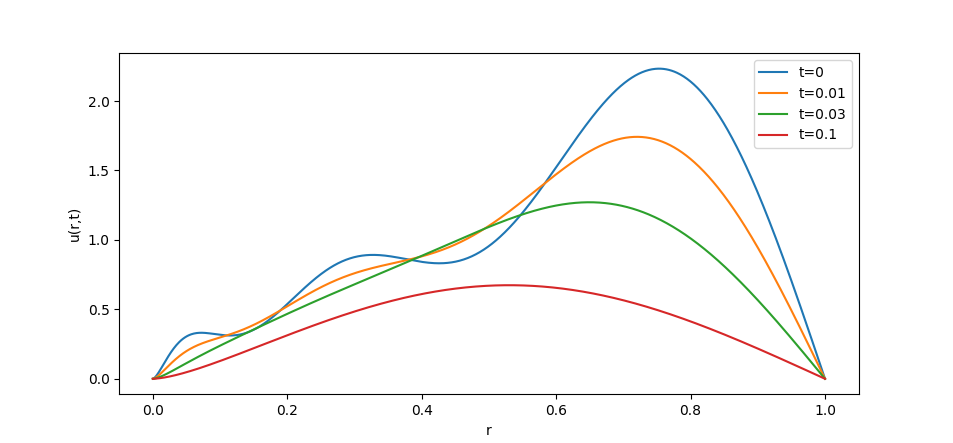
\includegraphics[width=0.8\textwidth]{1}
    \caption{Graph of first 5 terms over position}
    \label{fig:1}
\end{figure}

\begin{figure}[htpb]
    \centering
    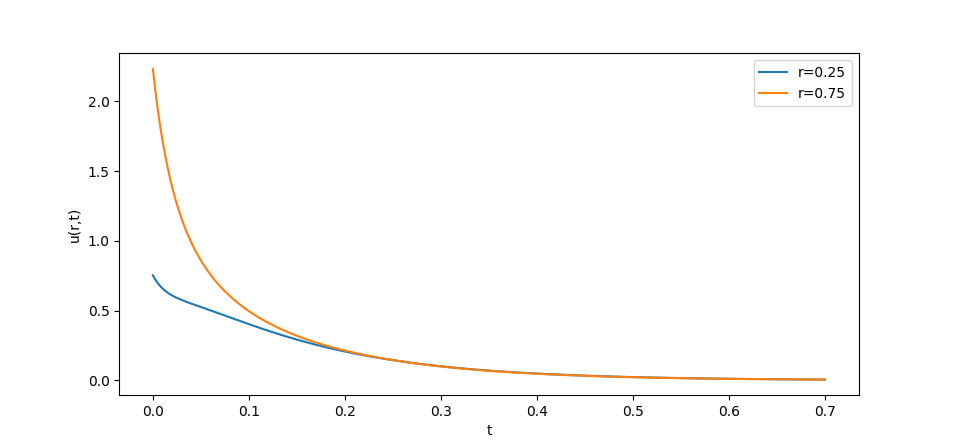
\includegraphics[width=0.8\textwidth]{2}
    \caption{Graph of first 5 terms over time}
    \label{fig:2}
\end{figure}

\end{document}
